\chapter{BACL-Streamer and Verification of the Unified Coordinate System}
\label{chpt:ver}

Insert text here

\section{Background}
\label{sec:ver-background}

Insert text here

Be sure to talk about IMMS here, as per discussion in \ref{chpt:integration}.

\section{Streamer v1.0}

Initial development of {\tt BACL-Streamer} began in 2009 with simple one-dimensional tests and demonstrations in Matlab, before moving to fully two-dimensional flows in the latter half of that year. Development continued until the Fall of 2010, when development began on v2.0.

v1.0 stored simulation variables, including conserved quantities, geometric coefficients, and grid motion parameters, as multidimensional arrays. To date, v1.0 has primarily served as a lessons-learned version, and informed many of the design choices in versions 2.0 and 3.0. 

\section{Streamer v2.0}
\label{sec:ver-Streamer2}

Development of {\tt BACL-Streamer} v2.0 began in 2010, and continued until moving to v3.0 in December 2011. It is most notable for its heavy use of Fortran object-oriented programming and for its implementation of the primary data structure as a linked list, rather than as an array. These design changes were made primarily as a means to improve on the performance of v1.0, which required extensive reallocation and copying of simulation data whenever grid points had to be added or removed. Unfortunately, many of these design changes also had a direct negative effect of simulation performance, and this, along with the need for a three-dimensional code and better verification options, led directly to the development of v3.0.

{\tt BACL-Streamer} v2.0 is structured as a group of interacting Fortran modules. It makes heavy use of object-oriented features introduced in Fortran 2003, including objects (Fortran derived types with bound methods), private variables, and the linked-list structure that replaces the multidimensional arrays used to store simulation variables in v1.0. 

\subsection{Node objects}
There are two fundamental objects used in v2.0: {\tt node} objects, which are containers for the simulation variables $p$, $\rho$, $u$, $v$, $A$, $B$, $L$, $M$, $x$, $y$, and so on, and the {\tt node\_array}, which is a linked list joining many nodes together into a two-dimensional grid. These two objects are fundamental to understanding the workings of v2.0, and their definitions are contained in {\tt types.f90}, and {\tt node\_array}, respectively. 

In addition to containing simulation variables, {\tt nodes} also provide a variety of functions and routines for working with {\tt node} objects directly, including arithmetic operators, and equivalence functions, and velocity component transformations. Additionally, each node contains pointers to each directly neighboring node, which are used to implement the linked list. 

The linked list itself requires more explanation. In this implementation, the list is built from a single head {\tt node} pointer, corresponding to the grid coordinates $i=1$, $j=1$. Specific nodes are accessed using the {\tt get\_node} function, which begins at the head and steps through the list to the appropriate node. {\tt set\_node} works in a similar fashion. The {\tt node\_array} module also contains a variety of functions that simplify the process of working adding and removing nodes, and populating them based on boundary conditions. 

Once the particulars of communicating with the linked-list structure are understood, the rest of v2.0 is a relatively straightforward implementation of the basic UCS algorithm. The driver program is the aptly named {\tt main.f90}, which reads a single input filename as a command line argument, initializes the simulation from this file using the {\\tt read\_boundary} subroutine, located in the {\tt boundary\_conditions\_init} module, and then calls the various modules of the code as necessary, until the desired output time has been reached. 

The {\tt read\_boundary} routine defines four {\tt boundary\_master} objects, defined in {\tt types.f90}, describing the left, right, bottom, and top boundary conditions, along with specifications for the computational region of interest, the dimensionality of the initial array, and the length of the computational differentials {\tt dxi} and {\tt deta}, as well as a variety of flags that are used to control various parts of the simulation. 

\section{Streamer v2.0 Verification}
\label{sec:ver-Str2-exact}

Verification is a critical piece in the development of any scientific code, and {\tt BACL-Streamer} v2.0 is no exception. As the code has no provision for the computation of source terms, as would be required for the method of manufactured solutions, verification is restricted to order-of-accuracy convergence using exact solutions to the Euler equations: a steady, supersonic Riemann problem, a wall-induced oblique shock, and a wall-induced Prandtl-Meyer expansion fan. 

\subsection{Two-dimensional Riemann problem}
\label{sec:ver-Str2-2dR}
The two-dimensional, steady, Riemann problem is a direct analogue to the one-dimensional, unsteady, Riemann problems that are discussed in Sec.~\ref{sec:UCS-Riemann}, and is especially useful as a verification test because of the stress it places on solvers. The particular problem used here is given by Hui\cite{Hui1999}, and consists of an expansion fan, a slip line, and a shock. These waves converge to a singularity located at the upstream boundary. The upstream conditions are given by:
\begin{equation}
\left(p,\rho,M,\theta\right)=\left\{
\begin{array}{lr}
\left(0.25,0.5,7,0\right) & :y>0\\
\left(1,1,2.4,0\right) & :y<0
\end{array}
\right.
\end{equation}
where $M$ is the flow Mach number and $\theta$ is the flow angle, measured from horizontal. This problem admits a similarity solution, much as the one-dimensional problem does, and the results from plotting this solution are shown in Figs.~\ref{fig:2.0-2d-riemann-density-0} and \ref{fig:2.0-2d-riemann-density-9}. In particular, it should be noted that the resolution of the slip line is greatly improved in the moving grid case. This is a well known effect of Lagrangian-esque simulations, and one of the beneficial features of UCS. 

\begin{figure}[p]
\centering
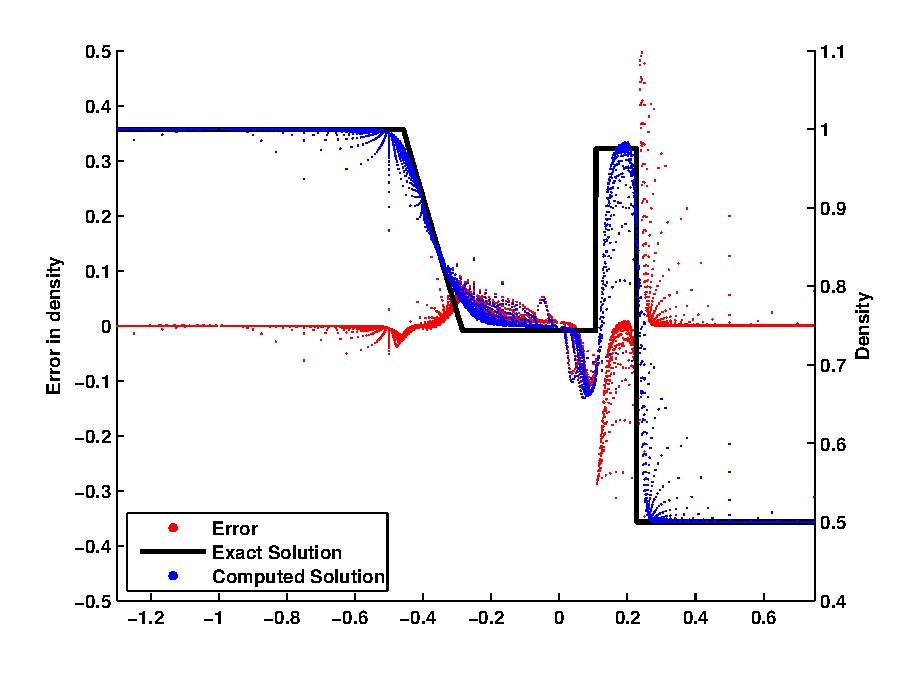
\includegraphics[width=\textwidth]{density_error_0.pdf}
\caption{The 2-D Riemann problem with corresponding numerical error, stationary grid}
\label{fig:2.0-2d-riemann-density-0}
\end{figure}
\begin{figure}[p]
\centering
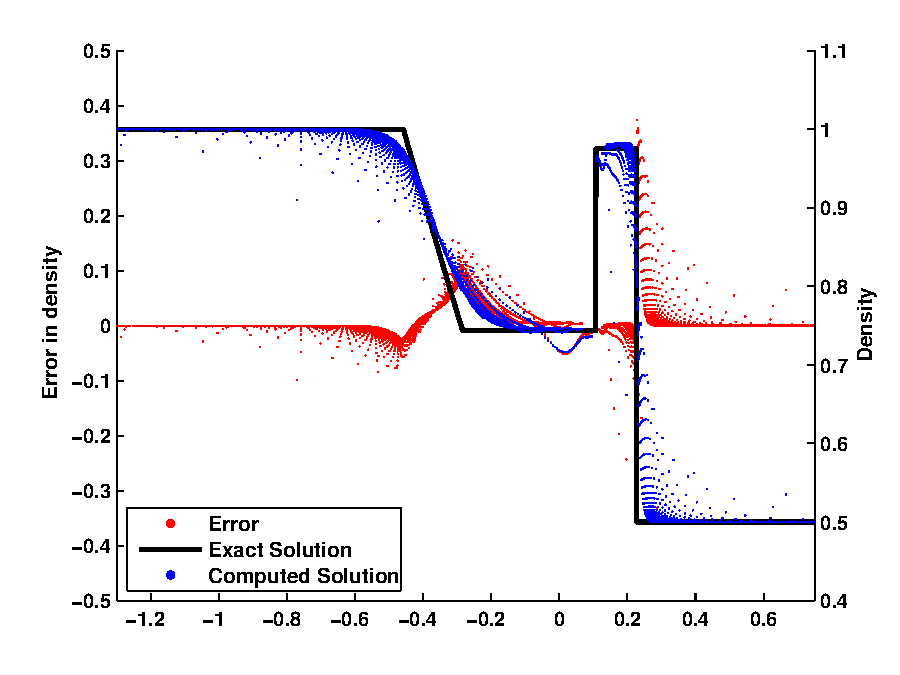
\includegraphics[width=\textwidth]{density_error_9.pdf}
\caption{The 2-D Riemann problem with corresponding numerical error, moving grid}
\label{fig:2.0-2d-riemann-density-9}
\end{figure}

The two-dimensional Riemann problem can be solved exactly\cite{Toro1994}, and so convergence rates can be measured for this problem. Convergence is tested for both moving and stationary grids, with and without the 2$^nd$-order MUSCL update. These convergence rates are shown in Fig.~\ref{fig:2.0-2d-riemann-convergence}. It is clear that the algorithm converges for at least three different test configurations, however this highlights one of the difficulties associated with convergence testing with shock-capturing codes, in that the presence of discontinuities generally reduces the observed order of convergence dramatically.\cite{Sabac1997}\cite{Popov2006} 

Unfortunately, these tests also expose drawbacks of the unified coordinates. 
While the moving grid simulation provides much higher accuracy at the slip line, overall accuracy actually decreases, and the rate of convergence drops measurably, as well. This may be due to the unsteady representation of the singularity at the upstream boundary. As the grid moves downstream, any point with an $x$ value that places it upstream of the boundary will have a state defined by the boundary conditions, while any with an $x$ value that places it downstream will be evolving in time. This effectively creates unsteadiness in the application of the singularity as the first grid points are located varying distances downstream of the boundary. The two-dimensional Riemann problem is defined entirely by that singularity, and unsteadiness could easily cause this increased error throughout the simulation. 

\begin{figure}[p]
  \centering
  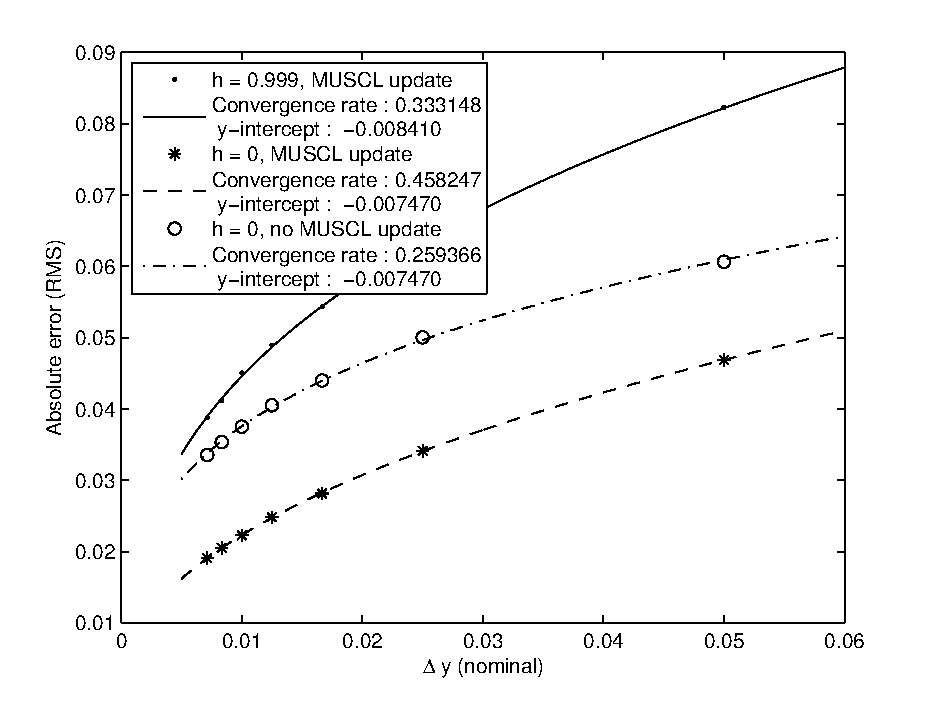
\includegraphics[width=\textwidth]{Riemann_convergence.pdf}
  \caption{Order of convergence $n$ of {\tt BACL-Streamer} v2.0 for a two-dimensional Riemann problem.}
  \label{fig:2.0-2d-riemann-convergence}
\end{figure}

\subsection{Wall-induced shock wave}
The next test was designed to provide better coverage of the different boundary conditions. Supersonic flow past a corner is well-defined, both for induced shocks and expansions, and provides a convenient test of solid wall boundary conditions. The upstream condition is given by:
\[
\left(p,\rho,M,\theta\right)=\left(1,1,1.8,0\right)
\]
The wall angle is chosen to yield a downstream flow angle of $45^o$. The grid is generated automatically, with grid velocity being set to 99.9\% of flow velocity ($h = 0.999$). Grid convergence rates again fall short of expectations. Like the Riemann problem, wall-induced shock flow is defined by the location of the critical point in the wall boundary condition, and it is unsurprising that an unsteady apparent location for this critical point would negatively affect error and convergence. 

\begin{figure}[p]
  \centering
  \caption{Root-mean-squared error for the oblique shock problem. The appearance of grid instabilities leads to two distinct error curves with different rates of convergence $n$.}
  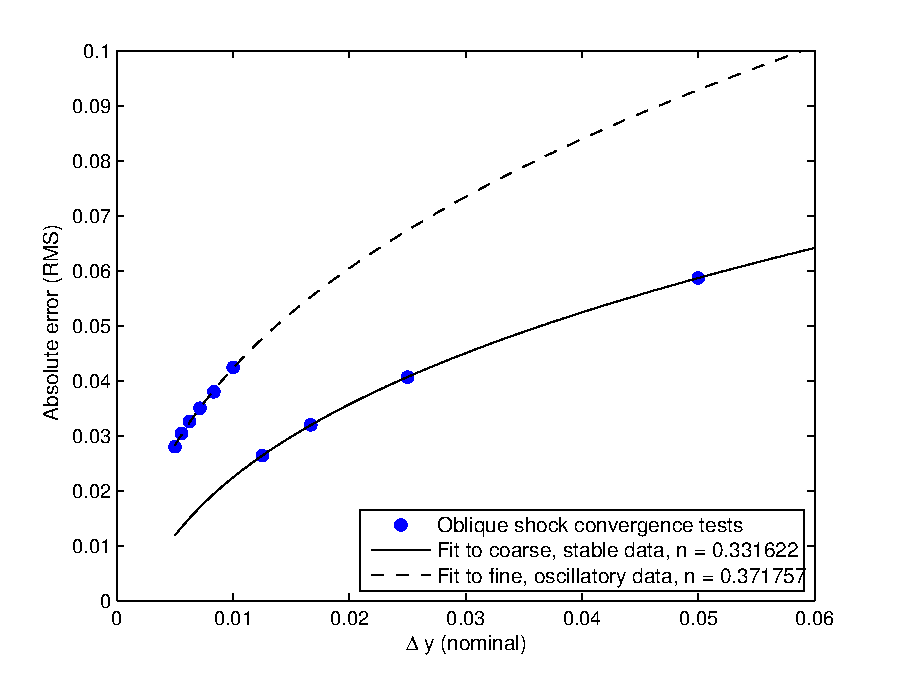
\includegraphics[width=\textwidth]{shock_convergence.pdf} 
\end{figure}
\begin{figure}[p]
  \centering
  \caption{A plot of normalized error in pressure, highlighting the oscillations which propagate downstream from the oblique shock.}
  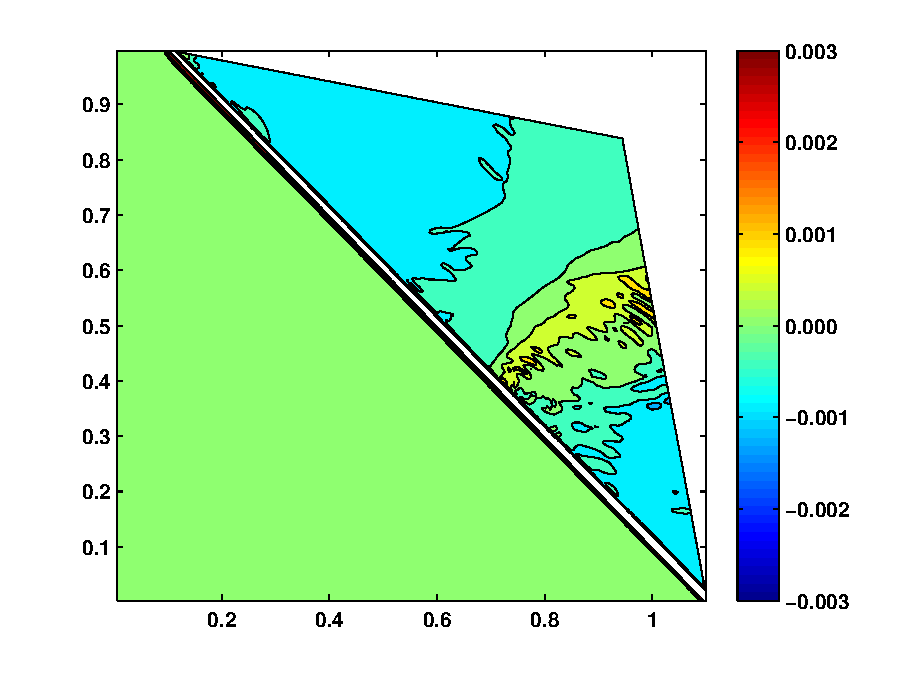
\includegraphics[width=\textwidth]{shock_instabilities.pdf}
\end{figure}

\subsection{Wall-induced expansion}
Wall-induced expansion fans, in contrast, offer a smooth solution, though one that is also dependent on a single critical point. Convergence rates were measured as with the shock, and with similar results, as seen in Fig.~\ref{fig:expansion-convergence}. A study was also done on flow behavior under varying expansion angles, which yielded important insights.  In the presence of strong expansion waves, the computational grid tends to pull away from the wall, as seen in Fig.~\ref{fig:expansion-separation}. 

\begin{figure}[p]
  \centering
  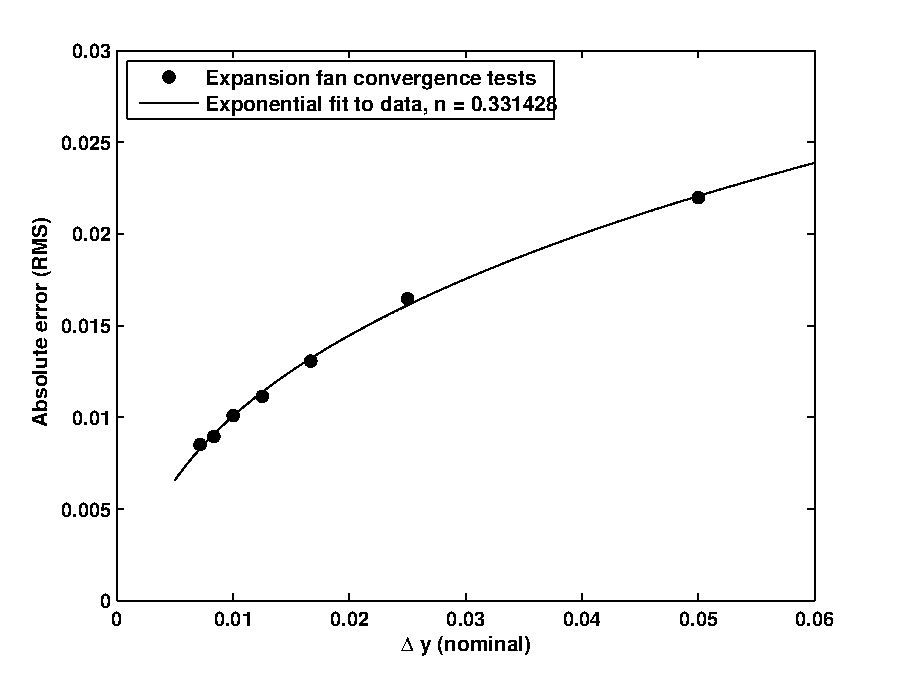
\includegraphics[width=\textwidth]{fan_convergence.pdf} 
  \caption{Root-mean-squared error for the Prandtl-Meyer expansion, with order of convergence $n$.}
  \label{fig:expansion-convergence}
\end{figure}

\begin{figure}[p]
  \centering
  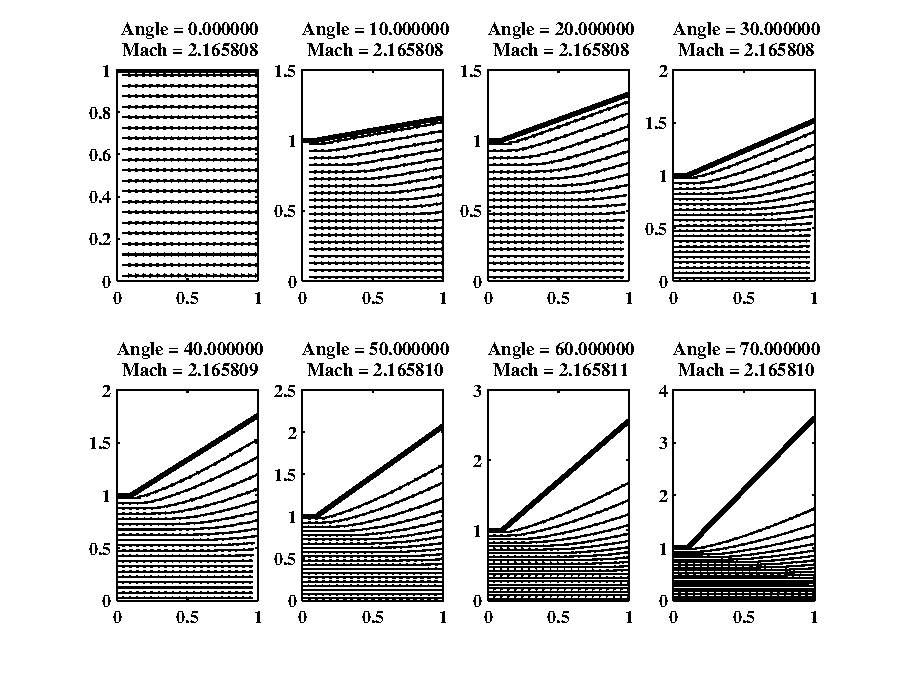
\includegraphics[width=\textwidth]{Expansion.pdf} 
  \caption{Computed streamlines for Prandtl-Meyer expansion at increasing expansion angles. Angles are given in degrees. }
  \label{fig:expansion-separation}
\end{figure}

\subsection{Conclusion}
Overall, this type of verification has highlighted the difficulties that must be overcome by any UCS program. Moving grids are not a simple thing to implement, especially when combined with problems that depend on the precise resolution of singular points. However, the increase in error is seen to be quite small, and the simplicity of the grid generation process in UCS may well be worth sacrifices in accuracy.

Unfortunately, it was impossible to conclusively establish verification for {\tt BACL-Streamer} v2.0. The available verification solutions simply incorporated too many difficult features, and it was impossible to separate errors due to the solution algorithm from errors due to the implementation of boundary conditions or errors in the coding itself. To solve this problem, it was necessary to turn to the method of manufactured solutions. This, along with the performance issues encountered in v2.0 and the need for a three-dimensional solver, led directly to the development of v3.0.

\section{Streamer v3.0}
\label{sec:ver-Streamer3}

{\tt BACL-Streamer}v3.0 was developed to remedy many of the difficulties encountered during development of version 2.0. It abandoned the object-oriented style, and reverted to the use of multidimensional arrays to track flow states. It is also the first version to attempt to handle the increasingly difficult problem of boundary condition specification and implementation, while also building a fully three-dimensional framework for later expansion. Finally, v3.0 is the first version to include modern software quality controls, including an expansive suite of unit tests and built-in order-of-accuracy convergence testing. Development was begun in late 2011, and has continued to the present time. 

{\tt BACL-Streamer}v3.0 can be roughly divided into two parts: a high-performance core, and developer-friendly scripts. The interface between these divisions is roughly equivalent to a division between the time-marching step, which is handled in script, and the space-marching computations, which are handled in core. Within a given time step, core functionality may be used extensively, but everything else is handled at the scripting level. The decision was made early in development to implement these as a hybrid Fortran/Python code, with the core being developed in Fortran 90, and the scripts developed in Python 2.x. The interface between the core and the scripts is provided by the {\tt f2py} package, which is included as part of the SciPy Python library. 

\subsection{Software prerequisites}

{\tt BACL-Streamer} v3.0 has made a concerted effort to leverage available software tools, while minimizing the number of special software packages that are required. Unfortunately, as of this writing, several of these packages provide required functionality only in the development branch, and so it is necessary to compile them from the {\tt git} repositories. This is noted, when applicable.

\begin{itemize}
\item Build tools
  \begin{itemize}
  \item Fortran90 compiler, such as GNU Fortran 4.2.3 (OS X).
  \item C compiler, such as Apple LLVM version 5.1.
  \item lapack library (required for test routines)
  \item standard GNU build tools e.g. {\tt make}, {\tt ar}, etc.
  \end{itemize}
\item Python environment
  \begin{itemize}
  \item Python 2.7.x
  \item SciPy library, for numerical integration. This functionality is currently available only on the {\tt master} branch, currently slated for v0.15, so SciPy must be built from source.
  \item NumPy package for array-based computation in Python. Version must be sufficiently new to build SciPy master, such as v1.8.1.
  \item Cython package, required to build NumPy and SciPy.
  \item Sympy package for use with manufactured solutions. Must also be built from the git development branch, currently v0.7.5.
  \item Nose testing package, useful for ensuring proper build of SciPy and Sympy.
  \end{itemize}
\end{itemize}

The build process will also compile several files from the {\tt MINPACK} library, which are used for some tests. These are distributed with the package, and so are not considered prerequisites. 

\subsection{Fortran core}

The Fortran Core itself consists of three main sections. There are the underlying library functions which solve Riemann problems, implement the Godunov method, and so on. There are the interface driver functions, which are linked using {\tt f2py} and provide the primary access to the library. Finally, there are the test functions, which implement everything from individual unit tests to full time-dependent convergence testing of the UCS system. These three components are all built through the Makefile included in the Streamer source directory. 

The most important unit of data in the Fortran Core is the {\tt main\_data} array. This is a four-dimensional array of double-precision floating point numbers, and contains all of the most important information needed for solution of the Euler equations in unified coordinates. Each computational node stores a flow state, 
% MathType!MTEF!2!1!+-
% faaagCart1ev2aaaKnaaaaWenf2ys9wBH5garuavP1wzZbqedmvETj
% 2BSbqefm0B1jxALjharqqtubsr4rNCHbGeaGqiVu0Je9sqqrpepC0x
% bbL8FesqqrFfpeea0xe9Lq-Jc9vqaqpepm0xbba9pwe9Q8fs0-yqaq
% pepae9pg0FirpepeKkFr0xfr-xfr-xb9Gqpi0dc9adbaqaaeGaciGa
% aiaabeqaamaabaabaaGcbaGaaC4vamaaBaaaleaacaWGPbGaamOAai
% Aadugaaeqaaaaa!31F2!
${{\bf{W}}_{ijk}}$, 
represented by 21 distinct numbers (the innermost array dimension), corresponding to the variables $p$, $\rho$, $u$, $v$, $w$, $A$, $B$, $C$, $L$, $M$, $N$, $P$, $Q$, $R$, $U$, $V$, $W$, $x$, $y$, $z$, $J$. This is very nearly the minimum set of numbers required to define the system; $J$ can be computed from the metric components, but it is used so frequently that it is useful to maintain a copy. 

{\tt main\_data} is also sized to be larger than is needed for holding array data. Boundary conditions in {\tt BACL-Streamer} are implemented using ghost points, which requires that {\tt main\_data} be sized at least two points larger in every spatial array dimension, as shown in Fig.~\%\%. Implementing boundary conditions in this way greatly simplifies the Core, and allows the difficult task of implementing boundary conditions to be handled in Python.

\subsubsection{Core library}
{\tt libStreamer} is built using {\tt make all}, and provides everything from basic matrix operations, to special utilities for working with the UCS flow state vectors, to  solving Riemann problems, to using the Godunov method to advance a UCS state from one time step to the next. The files which are compiled into {\tt libStreamer} are:
\begin{itemize}
\item {\tt GeneralUtilities.f90} - Useful utilities for working with UCS flow states.
\item {\tt Riemann.f90} - The function {\tt riemann\_solve}, which solves one-dimensional UCS Riemann problems.
\item {\tt TimeAdvancementStuff.f90} - Utilities for managing the unsteady nature of UCS grids, as well as an I/O routine for interfacing with Matlab.
\item {\tt Godunov.f90} - The function {\tt prim\_update}, which advances a UCS flow state from one time step to the next.
\item {\tt FortranNormalVectors.f90} - Routines for use in applying solid wall boundary conditions. Experimental.
\item {\tt grid\_motion.f90} - Routines for solving the grid control equations. At present, only Eq.~\ref{eq:grid-angle-preserving-g} is implemented.
\end{itemize}

\subsubsection{Library interface}
Though the {\tt f2py} tool greatly simplifies the process of communicating data between Python and Fortran codes, it is nonetheless advantageous to restrict and simplify the interface between the two divisions as much as possible. Driver modules for the {\tt Godunov} and {\tt grid\_motion} modules provide this kind of interface, and all calls to the underlying library functions pass through these drivers. As this interface project is ongoing, no such drivers exist for the other library modules at present.

Control of the underlying library routines is provided by the integer {\tt options} array. The values of different elements of this array determine behaviors such as the particular Godunov algorithm to use, or the number of ghost points needed to specify boundary conditions. While the library remains under active development, the exact behavior of these options remains in flux, but a snapshot of various option values and their meanings may still be helpful.

{\tt Options meanings                                                               

 [1-2]: controls which prim\_update algorithm to use                            

 [3-5]: sets values for dxi, deta, dzeta (0=>1., 1=>0.5, 2=>0.25)              

 [6-7]: controls grid motion.                                                  

 [6  ]: 0=>Eulerian, 1=>Lagrangian-esque, 2=>Constant, 3=>Angle-preserving         

 [7  ]: h0 = (1=>.25, 2=>.5, 3=>.999)                                              

 [101]: reports how many boundary ghost points are present                     

 [102]: controls spatial order of accuracy                                     

 [104]: Controls type of time step (constant or CFL)                           

 [301]: Controls type of grid motion                                           

}

This form of algorithm control is crude, but highly extensible. It is assumed that a more user-friendly interface will eventually be implemented.

\subsubsection{Unit testing and library verification}

The most difficult part of any code development project is ensuring the correctness of the code. To this end, tests have been developed that provide extensive coverage of the {\tt libStreamer} functionality. As much as possible, these tests rely on mathematics to evaluate functionality directly. For instance, if a function computes the inverse of a matrix, then the matrix product of a random initial matrix and the result of that function should be the identity matrix. Where necessary, the tests may be written based on sample problems where the results are known. Finally, the testing library provides routines for testing the overall convergence of the Godunov solver to exact solutions to the Euler equations, and comparing the measured rate of convergence with that returned by other codes.

The test suite is composed of additional Fortran modules, one for each module being tested. These contain both a battery of tests and a routine for interpreting the error messages that might result. A test suite driver program is also available. Compilation and execution of the full testing executable is done by executing {\tt make check} in the Streamer source directory.

The coverage of the test suite has been made as broad as possible, but there are known areas where testing has not yet been possible. As of this writing, testing of the Euler equations, where the grid transformation is the identity, has been implemented and achieved up to order-of-accuracy convergence for one-dimensional problems. Visual checks show agreement for two-dimensional problems, as well. Testing of code behavior with non-trivial UCS components remains incomplete.

\subsection{Python scripts}

While the Fortran Core provides most of the basic functionality required for a working UCS code, Python scripting handles many of the more complex tasks. It consists primarily of two files: {\tt main.py}, which covers basic simulation initialization and time-stepping, and {\tt BoundaryConditions.py}, which is an experimental boundary conditions implementation. 

\subsubsection{main.py}
Execution of a simulation program from Python is done by running {\tt python main.py <input file>}. The script reads data from the input file, and then initializes {\tt Stream} objects based on that data. This object defines the simulation boundary conditions, as well as options that allow for control of how the object behaves. This design is chosen to allow for future expansion, including multiple streams that interact through boundary conditions, specification of different flow solvers, incorporation of non-conservative source terms, and so on. Each {\tt Stream} object also includes the required tools to advance its state from one time step to another.

Once any streams have been initialized with appropriate boundary conditions, initial conditions, and options, a time-stepping simulation is run to advance these streams forward. 

\subsubsection{Input files}
Input files for {\tt BACL-Streamer} are Python files. They must contain an importable {\tt init} function returning three objects:
\begin{itemize}
\item {\tt bounds\_init} - Used by {\tt BoundaryCondtions.py} to initialize {\tt Bounds} objects.
\item {\tt initial\_conds} - An array to initialize {\tt main\_data}. If empty, then boundary conditions are used for initialization.
\item {\tt stream\_options} - A Python dict, containing options, additional information, and other directives required by the {\tt Stream}. For instance, source functions for the method of manufactured solutions are included here. Also includes the {\tt solver\_options} array, which is passed to the Fortran Core.
\end{itemize}

For more information on the effects of these objects, consult the {\tt main.py} and {\tt BoundaryConditions.py} files.

\subsubsection{BoundaryConditions.py}
{\tt BoundaryConditions.py} is an experimental method for implementing boundary conditions in an extensible way. The module organizes boundary condition data into {\tt Patch} objects, which are themselves organized into {\tt Face} and {\tt Bounds} objects. 

Each {\tt Patch} represents a single, distinct, boundary condition, such as a planar wall with a specific normal vector, or a constant pressure boundary. These patches are organized into {\tt Face} objects, representing the six logical boundaries of the {\tt main\_data} array, and everything is brought together in the {\tt Bounds} object, one of which corresponds to a {\tt Stream}. 

{\tt BoundaryCondtions.py}, {\tt BoundaryConditionsStuff.f90}, and the code-generated {\tt FortranNormalVectors.f90} work together to implement various types of boundary conditions, with varying degrees of success. The most difficult problems are a direct result of the unsteady nature of the UCS grid, which makes it difficult to determine how to best assign grid points to the appropriate boundary patches. Research in this area is ongoing. 

\subsection{BACL-Manufactured and the method of manufactured solutions}
{\tt BACL-Streamer} v3.0 is also integrated with the {\tt BACL-manufactured} Python package. {\tt BACL-manufactured} is an add-on tool that greatly simplifies the process of computing source terms for use in the method of manufactured solutions using either differential or integral methods. 

In order compute source terms for use in the method of manufactured solutions, it is necessary to provide both the system of equations and the proposed manufactured solution. With these, it is possible to generate manufactured source terms for differential MMS, as well as the integrands required for computing integral source terms for integrative MMS. {\tt BACL-manufactured} provides the machinery to do this quickly and easily, as efficiently as possible.

The package defines a {\tt SympyEquation} base class to describe the behavior of both integral and differential balance laws. This class provides the following methods for computation of source terms:
\begin{itemize}
\item {\tt balance\_diff} - Returns symbolic representation of differential manufactured source terms.
\item {\tt balance\_lambda\_init} - Returns the manufactured source terms from {\tt balance\_diff} as a Python lambda function.
\item {\tt balance\_integrate} - Returns integral form of manufactured source terms, integrated over some specified volume.
\end{itemize}
A {\tt SympyEquation} object is instantiated with a Python {\tt dict} containing Sympy representations of the integration variables, the manufactured solution to be used in computing the source terms, and symbolic representations of any discontinuities the solution contains. 

The {\tt SympyEquation} class is a general-purpose class, and is not intended for direct use. Instead, subclasses are used to define the equations for flux and source terms. Implementations are available for the linear heat equation and for the UCS Euler equations. These subclasses, along with a selection of appropriate manufactured solutions, are provided in equation-specific modules. This allows for easy expansion of the method to different equation sets. 

{\tt BACL-Streamer} also provides the {\tt integration} module, which is a collection of tools used to efficiently evaluate multidimensional integrals based on symbolic integrands with known discontinuities. The numerical methods used are discussed in detail in Section \ref{sec:int-nquad}, so the discussion here is limited to the manipulations required to derive integrals of the appropriate form for evaluation using {\tt nquad}. 

Given a symbolic representation of the flux and source vectors, as well as a particular manufactured solution, it is a simple matter to compute symbolic representations of the functions which must be integrated. The {\tt integration} package uses Sympy tools to convert these symbolic integrands to more computationally efficient Python functions, with an additional option to generate C functions. 

Finally, the package also processes any symbolic discontinuities into the appropriate form for the numeric integration routine, as described in Section \ref{sec:int-disc-tracking}. The end result is a complete set of functions defining the critical surfaces of integration.

Once all of this functional machinery has been initialized, the {\tt balance\_integrate} function provided by the {\tt SympyEquation} object can be called to evaluate the integral numerically, the results of which become the integrated source terms for use with integral manufactured solutions.

\section{Streamer v3.0 Verification}
\label{sec:ver-MMS}

Verification of {\tt BACL-Streamer} v3.0 is ongoing, and has been done only in preliminary cases for the basic Euler equations. Moving grids have not been verified as yet. The discussion here of integrative manufactured solutions relies heavily on the use of fast, accurate methods for evaluation of multidimensional integrals subject to discontinuities, discussed in detail in Chapter \ref{chpt:integration}. 

Because it was designed to incorporate non-conservative, manufactured solutions, {tt BACL-Streamer} v3.0 includes functionality for the inclusion of manufactured source terms as part of the time-stepping scheme in {\tt main.py}. The resulting equations are solved using a partial-time-step scheme similar to the dimensional splitting approximations, and described in Toro\cite{Toro2009}. Differential source terms are incorporated using SciPy's ODE solvers, while integral source terms are treated exactly like the existing flux integrals. 

To provide comparable testing with a different, though similar code, verification was also performed on Toro's NUMERICA\cite{Toro2009}\cite{Toro1999}. As the NUMERICA library does not allow for non-conservative source terms, it is verified against the exact, one-dimensional Riemann problem given by the initial states
% MathType!MTEF!2!1!+-
% faaagCart1ev2aaaKnaaaaWenf2ys9wBH5garuavP1wzZbqedmvETj
% 2BSbqefm0B1jxALjharqqtubsr4rNCHbGeaGqiVu0Je9sqqrpepC0x
% bbL8FesqqrFfpeea0xe9Lq-Jc9vqaqpepm0xbba9pwe9Q8fs0-yqaq
% pepae9pg0FirpepeKkFr0xfr-xfr-xb9Gqpi0dc9adbaqaaeGaciGa
% aiaabeqaamaabaabaaGceaGabeaacaWHxbGaeyyyIO7aaeWaaeaaca
% WGWbGaaiilaiabeg8aYjaacYcacaWG1baacaGLOaGaayzkaaaabaGa
% aC4vamaaBaaaleaacaWGmbaabeaakiabg2da9maabmaabaGaaGymai
% aac6cacaaIWaGaaiilaiaaykW7caaMc8UaaGymaiaac6cacaaIWaGa
% aiilaiaaykW7caaMc8UaaGimaiaac6cacaaIWaaacaGLOaGaayzkaa
% aabaGaaC4vamaaBaaaleaacaWGsbaabeaakiabg2da9maabmaabaGa
% aGimaiaac6cacaaIXaGaaiilaiaaykW7caaMc8UaaGimaiaac6caca
% aIXaGaaGOmaiaaiwdacaGGSaGaaGPaVlaaykW7caaIWaGaaiOlaiaa
% icdaaiaawIcacaGLPaaaaaaa!5DD0!
\[\begin{array}{c}
{\bf{W}} \equiv \left( {p,\rho ,u} \right)\\
{{\bf{W}}_L} = \left( {1.0,\,\,1.0,\,\,0.0} \right)\\
{{\bf{W}}_R} = \left( {0.1,\,\,0.125,\,\,0.0} \right)
\end{array}\]
The solution to this problem is readily obtained by reference to the discussion in Section \label{sec:UCS-Riemann}, or a numerical solution may be obtained from the Riemann solver used in the Godunov algorithm. 

{\tt BACL-Streamer} v3.0 was tested against the two-dimensional Riemann problem of Section \ref{sec:ver-Str2-2dR}, as well as the two different manufactured solutions. The first was given by:
% MathType!MTEF!2!1!+-
% faaagCart1ev2aaaKnaaaaWenf2ys9wBH5garuavP1wzZbqedmvETj
% 2BSbqefm0B1jxALjharqqtubsr4rNCHbGeaGqiVu0Je9sqqrpepC0x
% bbL8FesqqrFfpeea0xe9Lq-Jc9vqaqpepm0xbba9pwe9Q8fs0-yqaq
% pepae9pg0FirpepeKkFr0xfr-xfr-xb9Gqpi0dc9adbaqaaeGaciGa
% aiaabeqaamaabaabaaGcbaGaamiCaiabg2da9iabeg8aYjabg2da9i
% aadwhacqGH9aqpcaWG2bGaeyypa0Jaam4Daiabg2da9iaaigdacaGG
% UaGaaGymaiabgUcaRiaaicdacaGGUaGaaGynaiGacogacaGGVbGaai
% 4CamaabmaabaWaaSaaaeaacaaIYaGaeqiWdaNaamiEaaqaaiaad6ea
% daWgaaWcbaGaamiEaaqabaaaaaGccaGLOaGaayzkaaaaaa!47FA!
\[p = \rho  = u = v = w = 1.1 + 0.5\cos \left( {\frac{{2\pi x}}{{{N_x}}}} \right)\]
This provides a smooth, yet non-physical, and provides an excellent test of the Euler solver with source terms. The second solution is similar, with an added discontinuous jump:
% MathType!MTEF!2!1!+-
% faaagCart1ev2aaaKnaaaaWenf2ys9wBH5garuavP1wzZbqedmvETj
% 2BSbqefm0B1jxALjharqqtubsr4rNCHbGeaGqiVu0Je9sqqrpepC0x
% bbL8FesqqrFfpeea0xe9Lq-Jc9vqaqpepm0xbba9pwe9Q8fs0-yqaq
% pepae9pg0FirpepeKkFr0xfr-xfr-xb9Gqpi0dc9adbaqaaeGaciGa
% aiaabeqaamaabaabaaGcbaGaamiCaiabg2da9iabeg8aYjabg2da9i
% aadwhacqGH9aqpcaWG2bGaeyypa0Jaam4Daiabg2da9iaaigdacaGG
% UaGaaGymaiabgUcaRiaaicdacaGGUaGaaGynaiGacogacaGGVbGaai
% 4CamaabmaabaWaaSaaaeaacaaIYaGaeqiWdaNaamiEaaqaaiaad6ea
% daWgaaWcbaGaamiEaaqabaaaaaGccaGLOaGaayzkaaGaey4kaSYaai
% qaaeaafaWabeGadaaabaGaaGimaaqaaiaacUdaaeaacaWG4bGaeyip
% aWZaaSGbaeaacaWGobWaaSbaaSqaaiaadIhaaeqaaaGcbaGaaGOmaa
% aaaeaacaaIXaaabaGaai4oaaqaaiaadIhacqGHLjYSdaWcgaqaaiaa
% d6eadaWgaaWcbaGaamiEaaqabaaakeaacaaIYaaaaaaaaiaawUhaaa
% aa!5772!
\[p = \rho  = u = v = w = 1.1 + 0.5\cos \left( {\frac{{2\pi x}}{{{N_x}}}} \right) + \left\{ {\begin{array}{*{20}{c}}
0&;&{x < {{{N_x}} \mathord{\left/
 {\vphantom {{{N_x}} 2}} \right.
 \kern-\nulldelimiterspace} 2}}\\
1&;&{x \ge {{{N_x}} \mathord{\left/
 {\vphantom {{{N_x}} 2}} \right.
 \kern-\nulldelimiterspace} 2}}
\end{array}} \right.\]
These two solutions are shown in Fig.~\ref{fig:manufactured-solutions}
\begin{figure}[p]
\label{fig:manufactured-solutions}
\centering
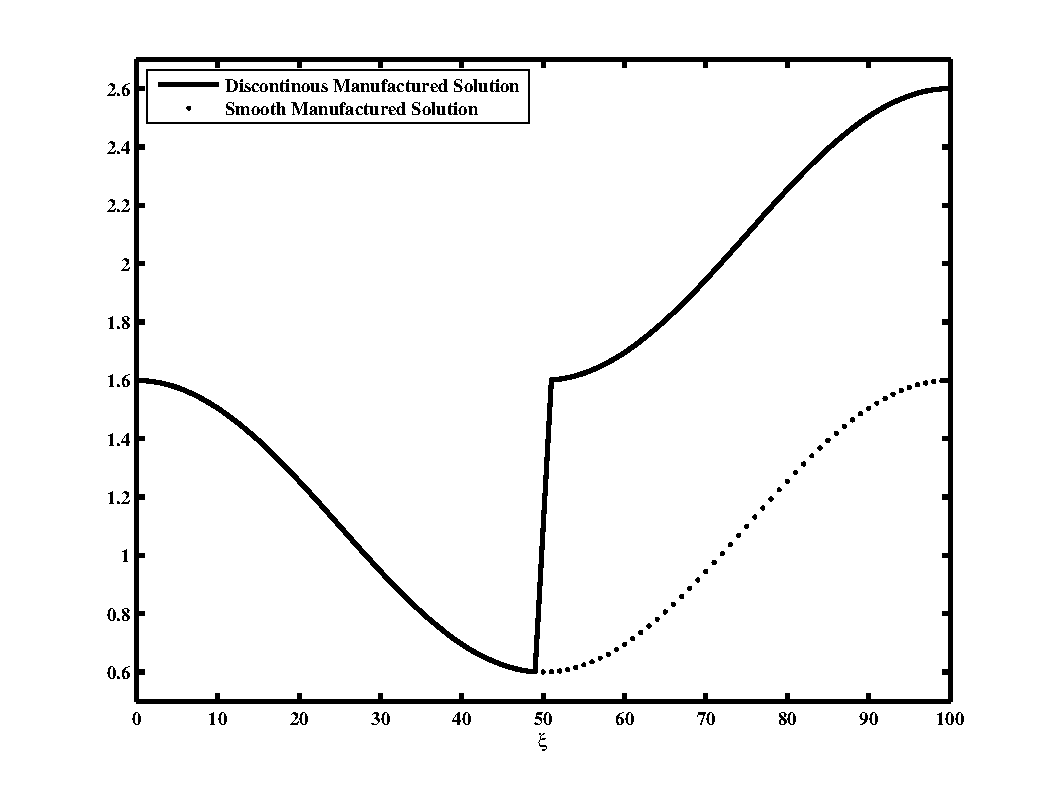
\includegraphics[width=\textwidth]{Manufactured_Solutions.pdf}
\caption{Manufactured solutions used for verification of {\tt BACL-Streamer} v3.0}
\end{figure}

In all, five different verification tests were run, as parameterized in Table \ref{tab:v3.0-convergence}. Measurement of a code's order of convergence requires the use of multiple grids at different levels of refinement. For structured grids, such as those used in BACL-Streamer, it is a simple matter to begin with a fine grid, and obtain coarser grids by neglecting multiples of two, three, etc. or else to obtain a finer grid by doubling the number of points. For the manufactured solutions, the baseline grid had 101 points, and coarsened this to obtain 51-, 26-, and 21-point grids corresponding to $\Delta x=1,2,4,5$, respectively. For the exact Riemann problem, a 101-point base grid is used to define 201- and 51-point grids, such that $\Delta x = 0.005, 0.01, 0.02$. For the two-dimensional, steady, Riemann problem, the initial grid is sized $60\times100$ with $\Delta x=\Delta y=0.01$, which is used to derive $30\times50$ and $120\times200$ grids, with $\Delta x=\Delta y=0.02,0.005$, respectively. 

\begin{tabular}[]{|p{1.7in}|p{1.2in}|p{1.43in}|p{.8in}|}
\label{tab:v3.0-convergence}
%\hline
 & Differential steps & Grid sizes & $x \times y$ ranges\\
\hline

Smooth, differential, manufactured solution & $\Delta x=1, 2, 4, 5$&
$nx = 101, 51 ,26 ,21$& $\{0, 100\}$\\
\hline

Smooth, integral, manufactured solution & $\Delta x = 1, 2, 4, 5$&
$nx=101, 51, 26, 21$&$\{0, 100\}$\\
\hline

Unsteady Riemann problem (NUMERICA)&$\Delta x = 0.005, 0.01, 0.02$&
$nx=201, 101, 51$&$\{0, 1\}$\\
\hline

Discontinuous, integral, manufactured solution & $\Delta x = 1, 2, 4, 5$ &
$nx=101, 51, 26, 21$&$\{0, 100\}$\\
\hline

Two-dimensional, steady, Riemann problem&$\Delta x=\Delta y=0.005, 0.01, 0.02$&
$nx\times ny=30\times50, \newline 60\times100, 120\times200$&
$\{0, 0.6\}\times\{-0.5, 0.5\}$\\
\hline
\end{tabular}

Once the grids have been defined, numerical solutions were computed and compared to exact solutions. The RMS value of the pointwise-error is then used to fit the function $f\left(\Delta x\right)=A\Delta x^n$. The resulting fits and the functions that describe them are shown in Figs.~\ref{fig:smooth-manufactured-convergence} and \ref{fig:disc-manufactured-convergence}. The equation fits are also given in Table \ref{tab:v3.0-convergence-fits}

\begin{tabular}[]{|l|l|l|}
\label{tab:v3.0-convergence-fits}
%\hline
 & Function Fit&Convergence Rate\\
\hline
Smooth, differential, manufactured solution&
$y=8.9\times10^{-4}\Delta x^{0.76}$&0.76\\

Smooth, integral, manufactured solution&
$y=7.7\times10^{-4}\Delta x^{0.54}$&0.54\\

Discontinuous, integral, manufactured solution&
$y=0.13\left(\frac{\Delta x}{500}\right)^{0.56}$&0.56\\

Unsteady Riemann problem (NUMERICA)& $y=0.20\Delta x^{0.50}$&0.50\\

Steady, two-dimensional, Riemann problem& $y=0.20\Delta x^{0.28}$&0.28\\
\hline
\end{tabular}

\begin{figure}
\centering
\label{fig:smooth-manufactured-convergence}
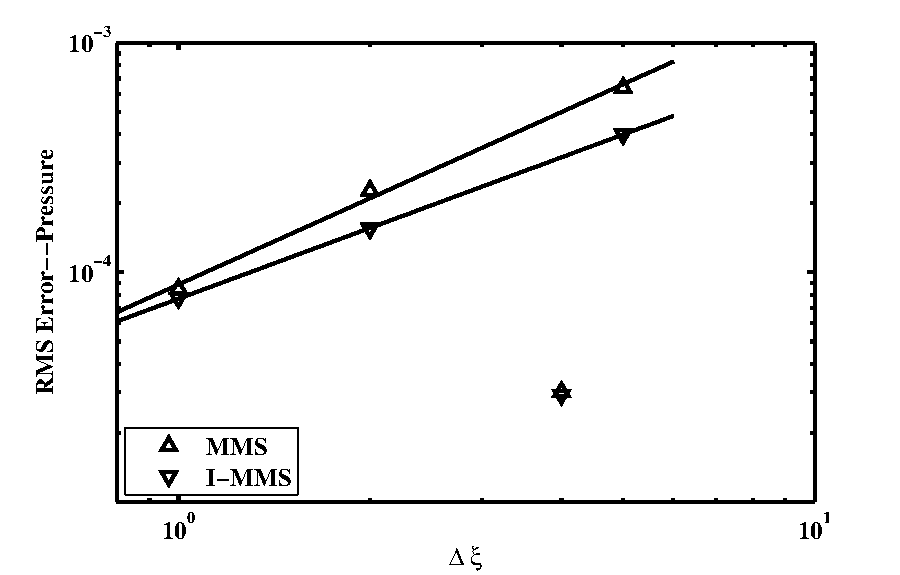
\includegraphics[width=\textwidth]{SmoothManufacturedConvergence_ppt.pdf}
\caption{Measured convergence rates for {\tt BACL-Streamer} v3.0 using both differential and integrative MMS with smooth manufactured solutions.}
\end{figure}

\begin{figure}
\centering
\label{fig:disc-manufactured-convergence}
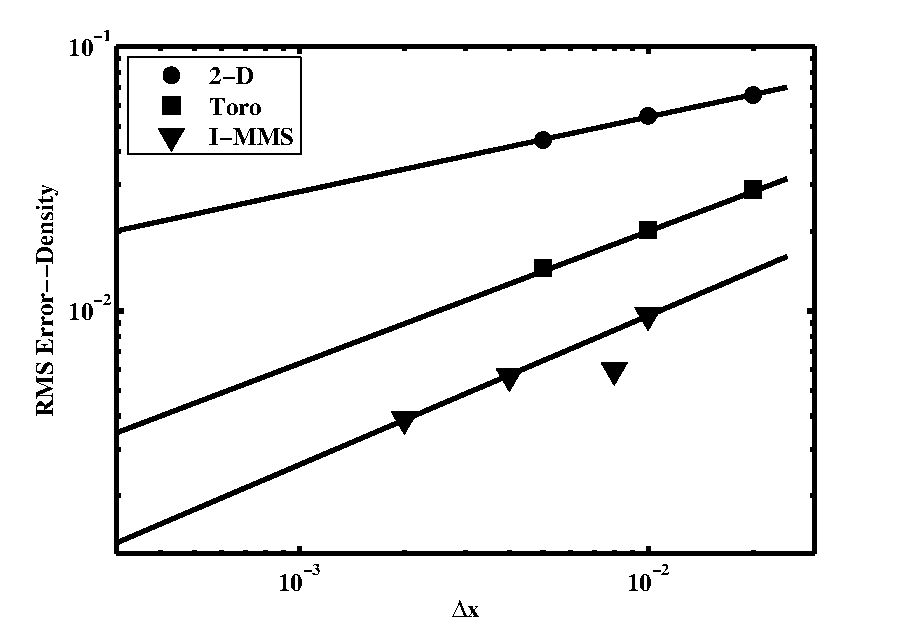
\includegraphics[width=\textwidth]{Disc_Combined.pdf}
\caption{Convergence rates for discontinuous solutions: the two-dimensional Riemann problem; the one-dimensional Riemann problem computed with Toro's NUMERICA; the discontinuous manufactured solution.}
\end{figure}

The convergence rates that result for differential MMS and integral MMS are quite comparable. The same agreement is seen when comparing the rate of convergence to discontinuous solutions, whether exact or manufactured. As before, a drop in convergence is observed for discontinuous solutions. 

\section{Future Work}
\label{sec:ver-future}
Preliminary results from verification of {\tt BACL-Streamer} v3.0 have been very encouraging, and provide confidence in the accuracy of the code within the coverage of the tests. The development of integrative manufactured solutions has opened many new doors, and allows for a truly thorough verification of both v3.0 and the UCS system as a whole. Beyond the scope of UCS, integrative manufactured solutions have the potential to revolutionize the entire field of code verification, in much the same way that traditional MMS has done in the last decade. 

The principal next steps for this work are a more complete code verification of {\tt BACL-Streamer} v3.0, followed by an in-depth investigation into the effects of using the UCS method to find solutions to fluid dynamical systems. The accuracy of the underlying time-step-eulerian approximation, the suitability of different boundary condition implementations, and the effects of different grid motion schemes, all need to be studied and understood, independently of the underlying flow solvers. This knowledge of how UCS affects simulation accuracy will guide the development of new solution algorithms, and it will provide designers with enough confidence in the method to use it on new projects.

